% fig_bilevel_game: the leader-follower game in one picture.
% Left: leader on top decides x, follower below answers with its best y(x).
% Right: a schematic of the leader's value c'x + d'y(x) as x varies (a staircase).
% Build: pdflatex fig_bilevel_game.tex   (6.5 in x 1.6 in)
\documentclass[tikz,border=2pt]{standalone}
\usepackage{mathptmx}
\usetikzlibrary{arrows.meta,calc}
\definecolor{leader}{HTML}{2A78D6}
\definecolor{follower}{HTML}{EB6834}
\definecolor{cert}{HTML}{1BAF7A}
\definecolor{ink}{HTML}{0B0B0B}
\definecolor{ink2}{HTML}{52514E}
\definecolor{muted}{HTML}{A9A8A2}
\definecolor{grid}{HTML}{E6E5E0}
\tikzset{
  every picture/.style={font=\fontsize{8}{9.6}\selectfont, color=ink, line cap=round},
  tier/.style={draw=#1, line width=0.9pt, fill=#1!9, rounded corners=4pt,
               minimum width=5.9cm, minimum height=1.05cm, align=center},
  flow/.style={-{Stealth[length=5pt,width=4pt]}, line width=0.9pt},
}
\begin{document}
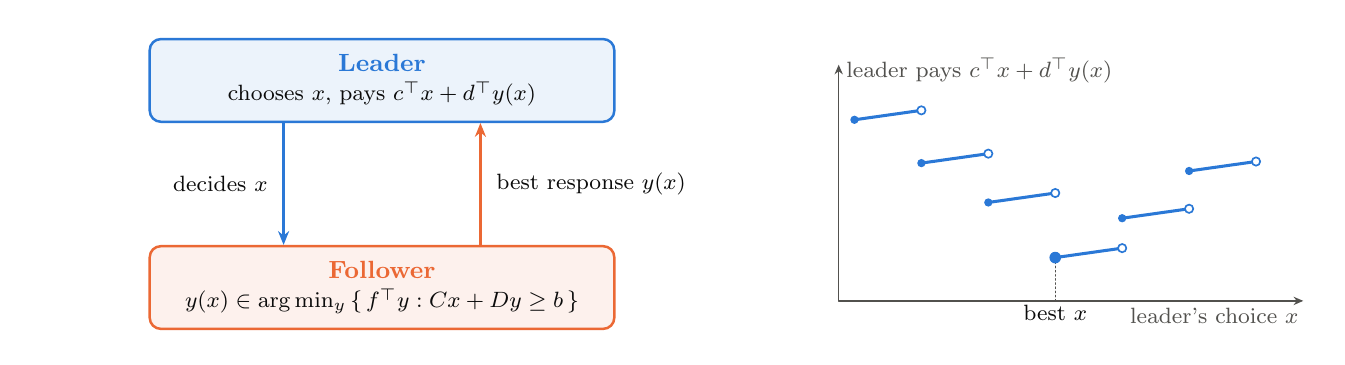
\begin{tikzpicture}
  % fixed page: 6.5 in x 1.6 in including the 2 pt border
  \useasboundingbox (0,0) rectangle (16.37,3.92);

  % ---- the two tiers ----
  \node[tier=leader] (L) at (4.5,3.25)
    {{\fontsize{9}{10}\selectfont\bfseries\color{leader}Leader}\\[1pt]
     chooses $x$, pays $c^\top x + d^\top y(x)$};
  \node[tier=follower] (F) at (4.5,0.62)
    {{\fontsize{9}{10}\selectfont\bfseries\color{follower}Follower}\\[1pt]
     $y(x) \in \arg\min_{y}\,\{\, f^\top y : Cx + Dy \ge b \,\}$};

  \draw[flow, leader]   ($(L.south)+(-1.25,0)$) -- ($(F.north)+(-1.25,0)$)
     node[midway, left=2pt, text=ink] {decides $x$};
  \draw[flow, follower] ($(F.north)+(1.25,0)$) -- ($(L.south)+(1.25,0)$)
     node[midway, right=2pt, text=ink] {best response $y(x)$};

  % ---- inset: the leader's value as a function of x ----
  \begin{scope}[shift={(10.3,0.45)}]
    \def\W{5.9}\def\H{3.0}
    \draw[ink2, line width=0.5pt, -{Stealth[length=3.5pt,width=3pt]}] (0,0) -- (\W,0)
      node[anchor=north east, inner sep=1.5pt, yshift=-1pt, text=ink2] {leader's choice $x$};
    \draw[ink2, line width=0.5pt, -{Stealth[length=3.5pt,width=3pt]}] (0,0) -- (0,\H)
      node[anchor=west, inner sep=1.5pt, xshift=1pt, yshift=-2pt, text=ink2] {leader pays $c^\top x + d^\top y(x)$};
    % staircase: pieces with slope c, jumps where the follower's reply changes
    \foreach \a/\b/\v in {0.2/1.05/2.30, 1.05/1.9/1.75, 1.9/2.75/1.25,
                          2.75/3.6/0.55, 3.6/4.45/1.05, 4.45/5.3/1.65}{
      \draw[leader, line width=1.1pt] (\a,\v) -- (\b,\v+0.12);
      \fill[leader] (\a,\v) circle (1.5pt);
      \draw[leader, fill=white, line width=0.6pt] (\b,\v+0.12) circle (1.5pt);
    }
    % the best choice
    \draw[ink2, densely dotted, line width=0.5pt] (2.75,0) -- (2.75,0.55);
    \fill[leader] (2.75,0.55) circle (2.1pt);
    \node[below, text=ink, inner sep=1.5pt] at (2.75,0) {best $x$};
  \end{scope}
\end{tikzpicture}
\end{document}
